\chapter{Binary sequence representation}
\label{kap:kap2}

This chapter is dedicated to outlining the current state of the bit vector
implementations. Bit vector stores binary sequence and supports methods $\access$,
$\rank$ and $\select$. As we have shown in section~\ref{section:WaweletTree}, wavelet
tree can be used to build a vector for the general alphabet using the bit vector
implementation. This is, why it is of the utmost importance to dedicate time
to creating fast and efficient bit vector implementation. We start with its
succinct representation, in which we simply store bits one after another. Then we
look at the compressed representation using the method RRR. In the end, we briefly
explain what other alternatives exist for compressed bit vector implementation.

\section{Bit vector implementation}

\subsection{Rank}
\label{section:rank}

Regarding $\rank$, we are concerned with two different methods namely $\rank_0(i)$
and $\rank_1(i)$. In every binary sequence, it holds that $$\rank_0(i) = i - \rank_1(i).$$
Thus, it is common to only provide
the implementation for one of them and answer the other one using this simple formula.
Let us now focus on a $\rank_1(i)$ method. There are two
straightforward solutions we can begin with to support $\rank_1$ on a bit vector~$B$.

The first solution does not use any precomputation at all. Every time we want
to compute $\rank_1(i)$, we go through all the bits preceding $i$-th and count all
the ones. This solution is not practical for longer bit vectors but it does not
add any additional space.

The second approach is to precompute $\rank$ of every bit. This enables us to answer
$\rank_1$ in constant time -- a single table lookup. However, the space needed to
support this solution is $\BigO(n\cdot\log n)$ bits where $n$ is the length of the
bit sequence.

\cite{gonzalez2005practical} combined these two solutions together to obtain an idea of a practically
interesting solution where we store the pre-computed $\rank_1$ values only for some
of the bits. At first, we choose a constant $k$ and split bit vector into non-overlapping
subsequences of $k$ bits. We name these subsequences \textit{superblocks}. We then
precompute $\rank_1$ only for the beginning of every superblock. Example of this
representation is presented in Fig.~\ref{obr:practicalRank}. This enables us to answer
$\rank_1$ in time $\BigO(k)$ as we need to only access the precomputed value and then count
bits from the start of the superblock up to the queried position. In this solution, we store
$\BigO(\ceil{n/k}\log n)$ bits of memory as there are $\ceil{n/k}$ superblocks and every rank
can be of size at most $n$. This version of the implementation allows us to balance between
speed and space usage using the parameter $k$. Increasing this parameter allows us to save
space. On the other hand, smaller $k$ requires less work to be done inside of the superblock.

In practice, the time of answering the query for smaller $k$ may be dominated by two cache misses
that most of the time occur when accessing the precomputed rank and then subsequently accessing
the bits on the beginning of the superblock. Subsequent continuous linear scan through bits in
one of the superblocks can then be very cache-friendly after the initial two cache misses and
thus very fast.

% TODO: moreover, bit operations - popcount
% TODO: in theory, for k ~ log n we already get linear space and \BigO(1) time if we assume a strong-enough model (RAM with log n bit registers with popcount)

\begin{figure}
	\begin{tabular}{c|c|c|c|c|}
	\cline{2-5}
	\textbf{B} & {\tt 0 0 1 0 1 1 0 1} & {\tt 1 1 1 0 1 1 1 1} & {\tt 0 0 0 0 0 1 1 0} & {\tt 1 1 0 0 1} \\ \cline{2-5}
	\end{tabular}

    \bigskip

    \begin{tabular}{c|c|c|c|c|}
        \cline{2-5}
        \textbf{precomputed ranks} & \tt 0 & \tt 4 & \tt 11 & \tt 13 \\ \cline{2-5}
        \end{tabular}

	\caption[TODO]{Example of dividing bit sequence $B$ into superblocks of length 8 and precomputing
    $\rank_1$ for the beginning of every superblock. Note that last superblock may not contain full
    number of 8 bits.}
	\label{obr:practicalRank}
\end{figure}

\paragraph{Constant time rank/sublinear extra space}

Although the previous solution works well and is commonly used in practice, it is possible to
answer $\rank$ query in constant time and only sublinear space overhead. It uses the partitioning first
used by \cite{okanohara2007practical}. We start as in the previous solution by splitting
the bit sequence into superblocks. This time we let the superblocks be of size $\log^2 n$
and again precompute $\rank$s for the beginning of every superblock. We further divide every
superblock into blocks of size $(\log n)/2$. We precompute $\rank$s for all of these
smaller blocks, but to save space, we only precompute it from the beginning of the corresponding
superblock.

Now, when queried for $\rank_1$ of some position, we combine:
1. Number of ones up to the beginning of its superblock.
2. Precomputed number of ones from the beginning of the superblock up to its block.
3. The number of ones that are before the queried position inside of its block (done by simple
table lookup in constant time).

The space overhead that this solution adds consists of three parts:
1. Precomputed $\rank$ for every superblock. Number of superblocks is $\BigO(n/\log^2 n)$
and we need $\BigO(\log n)$ bits to store every single $\rank$ value so the total amount is
\begin{equation}
    \BigO\left(\frac{n}{\log^2 n}\cdot \log n\right) = o(n).
    \label{eq:rank_space_1}
\end{equation}
2. Number of smaller blocks is $\BigO(n/\log n)$ but now, every block stores precomputed $\rank$ only from the
beginning of a superblock so this number is at most $\log^2 n$, so we need just $\BigO(\log\log^2 n)=\BigO(\log\log n)$
bits to store it. The total amount of space for the $\rank$s precomputed for smaller blocks is then
\begin{equation}
    \BigO\left(\frac{n}{\lg n}\cdot \log\log^2 n\right)=o(n).
    \label{eq:rank_space_2}
\end{equation}
3. The third part is the precomputed table where for every possible block and every
possible $\rank$, we store its result. There are only $2^{(\log n)/2} = \sqrt{n}$ blocks of length 
$(\log n)/2$. Number of possible $\rank$ queries over it is $\log n/2$ so this makes the table of the size
\begin{equation}
    \BigO(\sqrt{n}\cdot \log n\cdot \log\log n)
    \label{eq:rank_space_3}
\end{equation}
as every entry in the table needs at most $\BigO(\log\log n)$ bits of storage. The total space used for
this solution of $\rank$ is therefore sum of \ref{eq:rank_space_1}, \ref{eq:rank_space_2} and
\ref{eq:rank_space_3}, which is sublinear in $n$.

Although optimal in theory, this solution is not used in practice that much as it produces
3 cache misses and rather a complex implementation. One for accessing the precomputed rank up
to the start of the superblock, then another one for the precomputed value of rank to the
beginning of the block and in the end also one for accessing the precomputed $\rank$ value
of the block.

% TODO: ... depends on model... can be \BigO(k/w) if we consider RAM model with w-bit registers
% that supports popcount

\subsection{Select}
\label{section:select}

In case of a $\select$ over bit vector, we are again interested in two methods $\select_0$
and $select_1$. Although there is not a simple way how to convert the result of one to
another just like with $rank$, we shall be interested mainly in $select_1$ version as the
other one can be easily implemented using the same ideas. The important property of the
$\select$ method is that it works much like an inverse to $\rank$. This is given by the fact that
$$\rank_c(\select_c(i)) = i.$$

Thanks to $\rank$ being a nondecreasing function, it is possible
to binary search for the result of $\select_c(i)$ if we have an efficient implementation of
$\rank$. This can be nicely combined with the solution from the previous section.
At first, we binary search for the solution in the samples of $\rank$ stored in superblocks. When we
identify the correct superblock of length $k$ bits, we simply linearly scan for the solution. This
solution is not asking for any additional memory on top of the space used for $\rank$. The answer
can be given in time $\BigO(\log(n/k)+k)$. This solution even if not optimal works very well in
practice as observed by \cite{gonzalez2005practical} on bit vectors of length up to $2^20\approx 10^6$.

\paragraph{Constant time select}

There is also a constant time solution for $\select$ using the sublinear memory overhead.
The solution we are going to describe, proposed by \cite{clark1997compact}, is similar to
the solution for constant time $\rank$, based on a division to superblocks and blocks.

We begin by precomputing $select(i)$ for every $i$ that is a
multiple of $t_1=\log n/\log\log n$. These precomputed values take $\BigO(n/\log\log n)$ bits of space.
This process also splits the bit sequence into superblocks of possibly variable length such that
each superblock contains exactly $t_1$ ones (except possibly for the last).

There are now two categories of superblocks. The ones called \textit{long} that are of size bigger
than $t_1^2$. In these superblocks, we can store the positions of all ones as they are sparse
and there is not many of them as they are long. The total memory used is $\BigO((n/t_1^2)\cdot t_1\cdot
\log n) = \BigO(n/\log\log n)$.

The second type of superblocks shorter than $t_1^2$ called
\textit{short}. We apply the idea that we already used for the original bit sequence. Inside of
every short superblock, we precompute the $\select$ from the beginning of the superblock for every
multiple of $t_2=(\log\log n)^2$. These precomputed values are small as they only represent positions
from the beginning of a short superblock. Every one of these values takes $\log\log n$ of space so the
total amount of space used for the values is $\BigO(n/t_2\cdot \log\log n) = \BigO(n/\log\log n)$.

This breaks short superblocks into blocks. Again, each of these blocks except for maybe the
last one contains $t_2$ ones. For blocks of size bigger than $t_2^2$, we store the positions of all
ones as there are not many of these blocks and they are sparse. We may use the same reasoning as
in the previous part to conclude that this takes $\BigO(n/t_2^2\cdot t_2\cdot \log\log n) = \BigO(n/\log\log n)$
of bits. To take care of the blocks smaller than $t_2^2$ we can again precompute a table of all
the possible ways how the block may look and all the possible $\select$ queries over it with
their result. This table is of size $$\BigO(2^{t_2^2}\cdot t_2^2 \cdot \log t_2) = o(n)$$
and this representation enables us to answer $\select$ in constant time.

When answering $select_1(i)$, we can easily find the location of right superblock. If this
is a long superblock, we just look at the precomputed positions of ones in the superblock.
The matter is more complicated if we fall into a short superblock. In this case, we find
the location of the correct block. If this is a long block, we can once again just look
at the position of one we are interested in. If it is a short block, we have the precomputed
table where we index with the block and the position of one in the block, we are interested in.

\section{Compressed representation}
\label{section:compressed_bv}

In the previous section, we showed how $\rank$ and $\select$ queries can be answered in constant
time with just sublinear space overhead. In this section, we show that it is possible to compress
the whole bit vector close to the zeroth order entropy while still keeping the constant time $\rank$
and $\select$.

We start with the introduction of RRR, data structure based on ideas of \cite{pagh2001low} and
\cite{raman2007succinct}. The main idea of RRR is to split the bit sequence into blocks of size
$b$ and then represent a block with $c$ ones using only $\ceil{\log {b \choose c}}$ bits as
there are ${b \choose c}$ combinations for positions of ones. The whole block can be then uniquely
represented as a pair $(c, o)$ where $c$ is the number of ones in the block, called \emph{class} and
$o$ is an offset of this block in a sequence of all the ${b \choose c}$ blocks in this particular class.
Even if the ordering of the blocks with the same class can be arbitrary, only lexicographical ordering
is heavily used in practice.

Now, for this structure to work, we need to find a way how to convert between the bit representation of
a block and its compressed form $(c, o)$. The process of obtaining $c$ and $o$ from the raw representation
of block is called \textit{encoding}. The opposite process is called \textit{decoding}. Although
we would like both processes to be fast, we do the encoding just once, at the initial construction
of the bit vector while decoding is done every time we are accessing a particular bit in $B$ so in practice
it is more important to optimise for decoding speed.

\paragraph{Block encoding/decoding}

For shorter block lengths, such as $b\leq 15$, it is reasonable to generate two helper tables $E$ and $D$.
Table $E$ used for the encoding, maps the block to its offset. The other table $D$ is two dimensional and
stores the bit representation of the block that is associated with pair $(c, o)$ on position $D[c][o]$.
Both these tables $E$ and $D$ can be precomputed by generating all the possible blocks in lexicographical
order. After this precomputation, the encoding and decoding of a block takes constant time.

For longer block lengths, it is impractical or even impossible to store huge helper tables. On the other
hand, bigger block sizes yield better compression rates because of smaller per block overhead. The need for
helper tables was overcome by \cite{navarro2012fast} who developed method of \textit{on the fly-decoding}.
This method relies on a bit by bit encoding and decoding of the block, taking $\BigO(b)$ time. While decoding,
we can compute on every position using simple combinatorics, how many blocks precede a given prefix and decide,
whether next bit should be 0 or 1.

\paragraph{Arrangment of encoded blocks}

In the previous paragraph, we showed how single block can be encoded and decoded. The next question is how the
encoded pairs representing blocks are arranged in memory. This arrangement should consider space efficiency
but also allow easy access to individual blocks of $B$. 

The main part of this representation comprises of two arrays $C$ and $O$ storing the classes and offsets of
the blocks, respectively. The array $C$ is an array of elements that are of fixed length. Every element takes
$\ceil{\log_2(b+1)}$ bits of space. The array $O$, on the other hand, is an array of elements of variable
size where the $i$-th element is $\ceil{\log_2{b\choose C[i]}}$ bits long. Note that accessing $i$-th element
in array $C$ is easier than doing the same in array $O$.

\paragraph{Accessing bits in RRR}

Accessing $x$-th bit of original sequence $B$ consists of three steps. The first is to obtain the
compressed representation of a block where $x$-th bit is located. The second step is to decode this block and
the third is to access the particular bit of interest in the decoded block. The $x$-th bit is contained in the
$i$-th block where $i=\floor{x/b}$. Its compressed representation is $(C[i], O[i])$.

Obtaining $C[i]$ is trivial as it is at the fixed memory offset from the beginning of array $C$. Getting the
value of $O[i]$ is harder as it is not at a known memory offset but it can be still expressed as
$$\sum_{j=1}^{i-1} \ceil{\log_2{b\choose C[i]}}$$. This can not be, however, computed in constant time without
any precomputed information and we need to basically one by one skip over elements that come before $O[i]$.
To access the $i$-th block, we need in the worst case to look at all the elements of $C$ and this
takes $\BigO(n/b)$ time. For now, we stay with this solution and analyze its space usage.

\paragraph{Space usage of RRR}

Our current representation needs to store the arrays $C, O$ and helper table $D$. Let us now
analyze the space used by these structures. $C$ is an array of $\ceil{n/b}$ elements of fixed size
$\ceil{\log(b+1)}$. For array $O$ we argue that its size is bounded by

\begin{align*}
    \sum_{i=1}^{n/b} \ceil{{\log b\choose c_i}}
    &\leq \sum_{i=1}^{\ceil{n/b}} \log {b\choose c_i} + \ceil{n/b} \\
    &= \log\prod_{i=1}^{\ceil{n/b}} {b\choose c_i} + \ceil{n/b} \\
    &\leq \log{n\choose \#_1(B)} + \ceil{n/b} &\leq nH_0(B) + \ceil{n/b}
\end{align*}

where $\#_1(B)$ denotes the total number of ones in $B$. We obtained (TODOsomeref) using the
observation that ${n\choose k} {m\choose \ell} \leq {n+m\choose k+\ell}$. This can be seen
when we interpret the left side of the equation as a number of ways we can choose $k$ elements
from $n$ elements and $\ell$ elements from another $m$ elements. This is all contained on the
right side of the equation that includes all these combinations. $D$ is storing $2^b$ entries
and each entry is using $b$ bits of storage. The total space used is then
$$nH_0(B) + \ceil{n/b} + \ceil{n/b} \cdot \ceil{\log(b+1)} + b2^b.$$ To speed up the process
of accessing block, we can store the pointers into every $k$-th element of $O$. The example of
this solution can be observed in Fig.~\ref{obr:RRRFinal}. This divides the process of locating
$O[i]$ into two parts. The first is to find the nearest pointer leading to element before $i$
and then move at most $k$ places. This additional structure of roughly $n/(bk)$ integers uses
$\BigO(\log(n)\cdot \frac{n}{bk})$ bits of space.

\begin{figure}
	\centerline{
		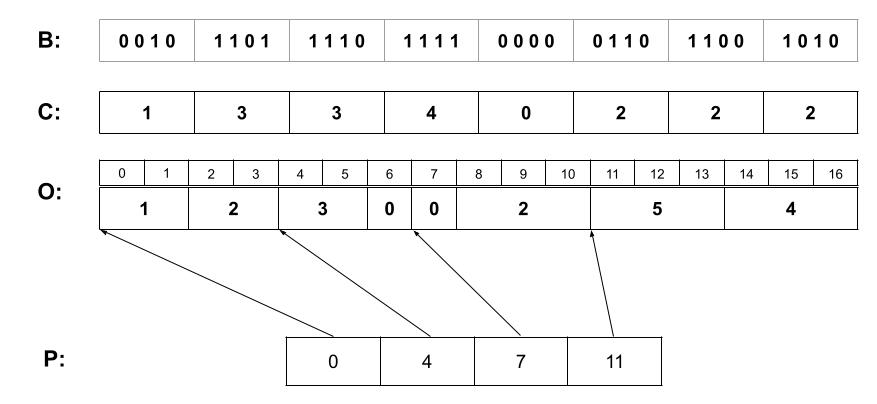
\includegraphics[width=0.9\textwidth, height=0.3\textheight]{images/rrr}
	}
	\caption[TODO]{RRR implementation. $B$ shows the original bit sequence cut to
    blocks. $C$ stores the class which is in this case number of ones in the block.
    $O$ uses variable number of bits per entry, in general, $i$-th entry uses
    $\ceil{\log_2{b\choose C[i]}}$ bits and stores the lexicographical order
    of this block in the class $C[i]$. For $k=2$ we can see a helper array $P$
    storing bit offsets into every $k$-th element namely $0, 2, 4\ldots$
	}
	\label{obr:RRRFinal}
	% source at https://docs.google.com/drawings/d/1f1M7e-dZIiIZh1RdgqnmptF3xWZBKqjms3f_aQwVMhg/edit
\end{figure}

When setting the block size to $\log(n)/2$ we obtain interesting practical results as
the total space used by our representation is equal to $nH_0(B) + o(n)$ bits. This means
that we are storing only a sublinear amount of data on top of the zeroth order empirical entropy.

When we are interested in obtaining the best practical results, block size becomes
one of the most important parameters of RRR implementation. As we shall show in the next
chapter, bigger block size is better because of lower per bit overhead. Also, not all block
sizes are used in practice. Very often, we are interested in block sizes of the form $2^k-1$.
This is because the number of ones in block of size $2^k-1$ can be number between 0 and $2^k-1$
making this in total $2^k$ possibilities. Storing this number in the fixed bucket of size
$k$ bits makes use of all the available space. This is why most commonly used bucket sizes in
practice are 15, 31, 63 and 127. For block size of 15 the encoding and decoding table
each occupies roughly 64kB of space. This is because every table consists of $2^{15}$ of entries
each taking 2 bytes of storage. Unfortunately, for block size of 31 these two tables would consume
roughly $2^{31}\cdot 4$ bytes of storage. That amounts to roughly 8.5GB of space and makes this approach
unusable in practice. This problem force us to use the on the fly decoding for block sizes
bigger than 15. The disadvantage of this approach is that it takes $\BigO(b)$ steps to decode the block.
Furthermore, on the fly decoding contains branches and it is hard to parallelize its steps in some meaningful
way. Overall, this makes the block size a parameter that we can adjust to balance between better space
efficiency and faster runtime performance.

\paragraph{Alternatives}
% https://github.com/simongog/sdsl-lite/blob/master/include/sdsl/sd_vector.hpp

So far we have provided just one example of the bit vector implementation.
RRR is used on sequences with low entropy, where the frequency of zeroes/ones
is shifted to one or the other side such as 20-40\% of all bits are the same.
There is also a second class of the bit vector implementations, heavily
used when the frequency of zeroes or ones is more significantly shifted.
Although we stated that RRR is used in case of shifted frequencies, when the number
of ones is very small, i.e. less than 5\% of the sequence, sparse bit vector
implementations may outperform solutions based on RRR as was observed by \cite{navarro2012fast}.
Where RRR stands out from some of its alternatives is that it is also very competitive
in cases where frequencies of zeroes and ones are similar globally, but the bit
sequence has a lot of places where locally zeroes or ones are over-represented.
Numerous sparse bit vector solutions are based on the work of \cite{okanohara2007practical}.